%% Factsheet template for AIM 2022 challenge
%% 
%%

\documentclass{article}

\usepackage{graphicx}
\usepackage{hyperref}
\usepackage{url}
\usepackage{colortbl, color, xcolor}
\usepackage{subcaption}

\title{NTIRE 2023 Real-Time Super-Resolution}

%%% Makre sure your teamname is short and does not contain special characters. It can also be the name of your method e.g. CompactSRNet - be more creative than use :)

%%% Add Your names and affiliations.
\author{\textcolor{red}{SEU\_CNII}\\
\textcolor{red}{Daheng Yin, Baijun Chen, Mengyang Liu}\thanks{\textcolor{blue}{School of Computer Science and Engineering, Southeast University}}\\
}


\begin{document}

\maketitle

This factsheet template is meant to structure the description of the contributions made by each participating team in the NTIRE 2023 Real-Time Super-Resolution Challenge.
%
The provided information, the codes/executables and the achieved performance on the testing data are used to decide the awardees of the NTIRE 2023 Real-Time Super-Resolution Challenge. 

\begin{enumerate}
    \item The models will be benchmarked as indicated in \url{https://github.com/eduardzamfir/NTIRE23-RTSR#evaluation-of-your-submission}.
    \item The test set is similar to the validation set, including only 4K native images. Reproducibility is a must. \textbf{We will only run and benchmark the models, we will not release or open-source them.} Open sourcing the solution is a must to receive the prizes, up to the team.
    \item The winners, the awardees and the top ranking teams will be invited to co-author the NTIRE 2023 Real-Time Super-Resolution Challenge report and to submit papers with their solutions to the NTIRE 2023 workshop. Detailed descriptions are much appreciated: brief description of all models and experiments tested, ablations, visualizations, things that did not work, datasets, pre-trained models, etc. You can share qualitative results via shared folder at google drive, dropbox, etc.
\end{enumerate}

\textbf{If you participate in both Track 1 and 2, you only need to submit 1 factsheet}.
This factsheet, and the source codes/models/executables (as specified \href{https://github.com/eduardzamfir/NTIRE23-RTSR#evaluation-of-your-submission}{here}) must be sent to \textbf{all of the NTIRE 2023 Real-Time Super-Resolution Challenge organizers} by email. We accept download links from your website, google drive, dropbox, etc. When using cloud services, please remember to allow sharing and consider the traffic limit of your service provider. If there is any problem, we will contact the team leader.

\begin{table}[h]
\begin{center}
\begin{tabular}{|c|c|}
    \hline
    Organizer name & Email \\
    \hline
    Marcos Conde  & marcos.conde@uni-wuerzburg.de  \\
    Eduard Zamfir & eduard-sebastian.zamfir@uni-wuerzburg.de  \\
    Radu Timofte  & radu.timofte@uni-wuerzburg.de \\
    \hline
\end{tabular}
\vspace{-0.5cm}
\end{center}
\end{table}
 \newpage
\section*{Email final submission guide}

\texttt{
To: marcos.conde@uni-wuerzburg.de, \\
eduard-sebastian.zamfir@uni-wuerzburg.de, \\
radu.timofte@uni-wuerzburg.de\\
cc: your\_team\_members\\
Title: NTIRE 2023 Real-Time Super-Resolution Challenge - TEAM\_NAME\\
}

Body contents should include: 

a) the challenge name (AND TRACKS): NTIRE 2023 Real-Time Super-Resolution Challenge

b) team name 

c) team leader's name and email address 

d) rest of the team members 

e) team name and user names on CodaLab competitions 

f) executable/models/source code attached or download links. We will run and benchmark the models following \url{https://github.com/eduardzamfir/NTIRE23-RTSR#evaluation-of-your-submission}.

g) factsheet attached. You can also provide a link to \textbf{overleaf}. Only we, the organizers, will be able to read it. Factsheet must be a compiled pdf file together with a zip with .tex factsheet source files (including figures with good resolution). 

\section{Team details}

\begin{itemize}
\item Team name: SEU\_CNII
\item Team leader name: Daheng Yin
\item Team leader institution and email: School of Computer Science and Engineering, Southeast University; yindaheng98@seu.edu.cn
\item Rest of the team members: Baijun Chen, Mengyang Liu
\item Team website URL (if any): N/A
\item Affiliations: School of Computer Science and Engineering, Southeast University
\item Usernames on the NTIRE 2023 Real-Time Super-Resolution Codalab leaderboard (development/validation and testing phases): yindaheng98
\item Link to the codes/executables of the solution(s) following \url{https://github.com/yindaheng98/NTIRE23-RTSR}
\end{itemize}

\section{Contribution details}

\begin{itemize}
\item Title of the contribution\\PRFDN: High Parallelism Distillation Network For Image Super-resolution
\item General method description (Summary)\\We proposed Parallel RFDN (PRFDN) based on the pre-trained RFDN\cite{liu2020residual} as is shown in figure \ref{fig:PRFDN}. Our method disentangles the sequentially computed trunks in RFDN into branches (figure \ref{fig:Branching}) and performs re-parametrization to make these branches inference in parallel on single devices. After that, we further perform pruning on the model (figure \ref{fig:Pruning}) and finetune it to achieve higher performance.
\item References: RFDN\cite{liu2020residual}, Torch-Pruning\cite{fang2023depgraph}
\item have you tested previously published methods? (yes/no) If yes, please specify which methods and the results/problems you found. N/A
\item Other methods and baselines tested (even if results were not top competitive). N/A
\end{itemize}

\section{Global Method Description}

We proposed Parallel RFDN (PRFDN) as is shown in figure \ref{fig:PRFDN}.
Our method consists of four stages to transform a pre-trained RFDN\cite{liu2020residual} into PRFDN.
\begin{enumerate}
    \item Branching. To accelerate the inference, we first consider reducing the data dependency in the model to achieve higher parallelism. Our method disentangles the sequentially computed trunks into branches. As is shown in figure \ref{fig:Branching}, after the branching, the major part of the model will consist of four independent branches that can calculate in parallel. To improve the accuracy, we also design a small SR block (SRFDB) based on the RFDB of RFDN and add them before the input of each branch. 
    \item Training. Since we only change the data flow but not the structure of RFDB, the pre-trained RFDN parameters can still be loaded into the major part of our branch model (only except for those SRFDBs). To benefit from the pre-training, we load the pre-trained RFDN parameters into our branch model before training our branch model.
    \item Re-parametrization. Without much data dependency, branches in our model can be computed in parallel. However, a single GPU cannot compute two or more different models in parallel. To address this issue and achieve parallel computing of multiple branches on a single GPU, we should merge the four branches into a single branch. As is shown in figure \ref{fig:Re-parametrization}, we realize that the major part of these four branches (RFDBs and SRFDBs) have exactly the same structure but different parameters, so we merge and re-parametrized the RFDBs and SRFDBs into a single branch. More specifically, we create a bigger RFDB and a bigger SRFDB with bigger convolution layers and move the weight and bias from the RFDBs and SRFDBs into them. After re-parametrization, we get a bigger model that is equivalent to that of the branches of the branch model computed in parallel on a single GPU.
    \item Pruning. The re-parametrized model is big. To further accelerate the inference, we applied channel pruning on our re-parametrized model, as is shown in figure \ref{fig:Pruning}. To accurately extract the channel dependency for pruning, we first replace each concatenate and split operation with an equivalent convolution operation. After replacement, we used Torch-Pruning\cite{fang2023depgraph} to prune the model and finetune the model between each pruning step.
\end{enumerate}

\begin{figure}
    \centering
    \begin{subfigure}[b]{0.49\linewidth}
		\centering
        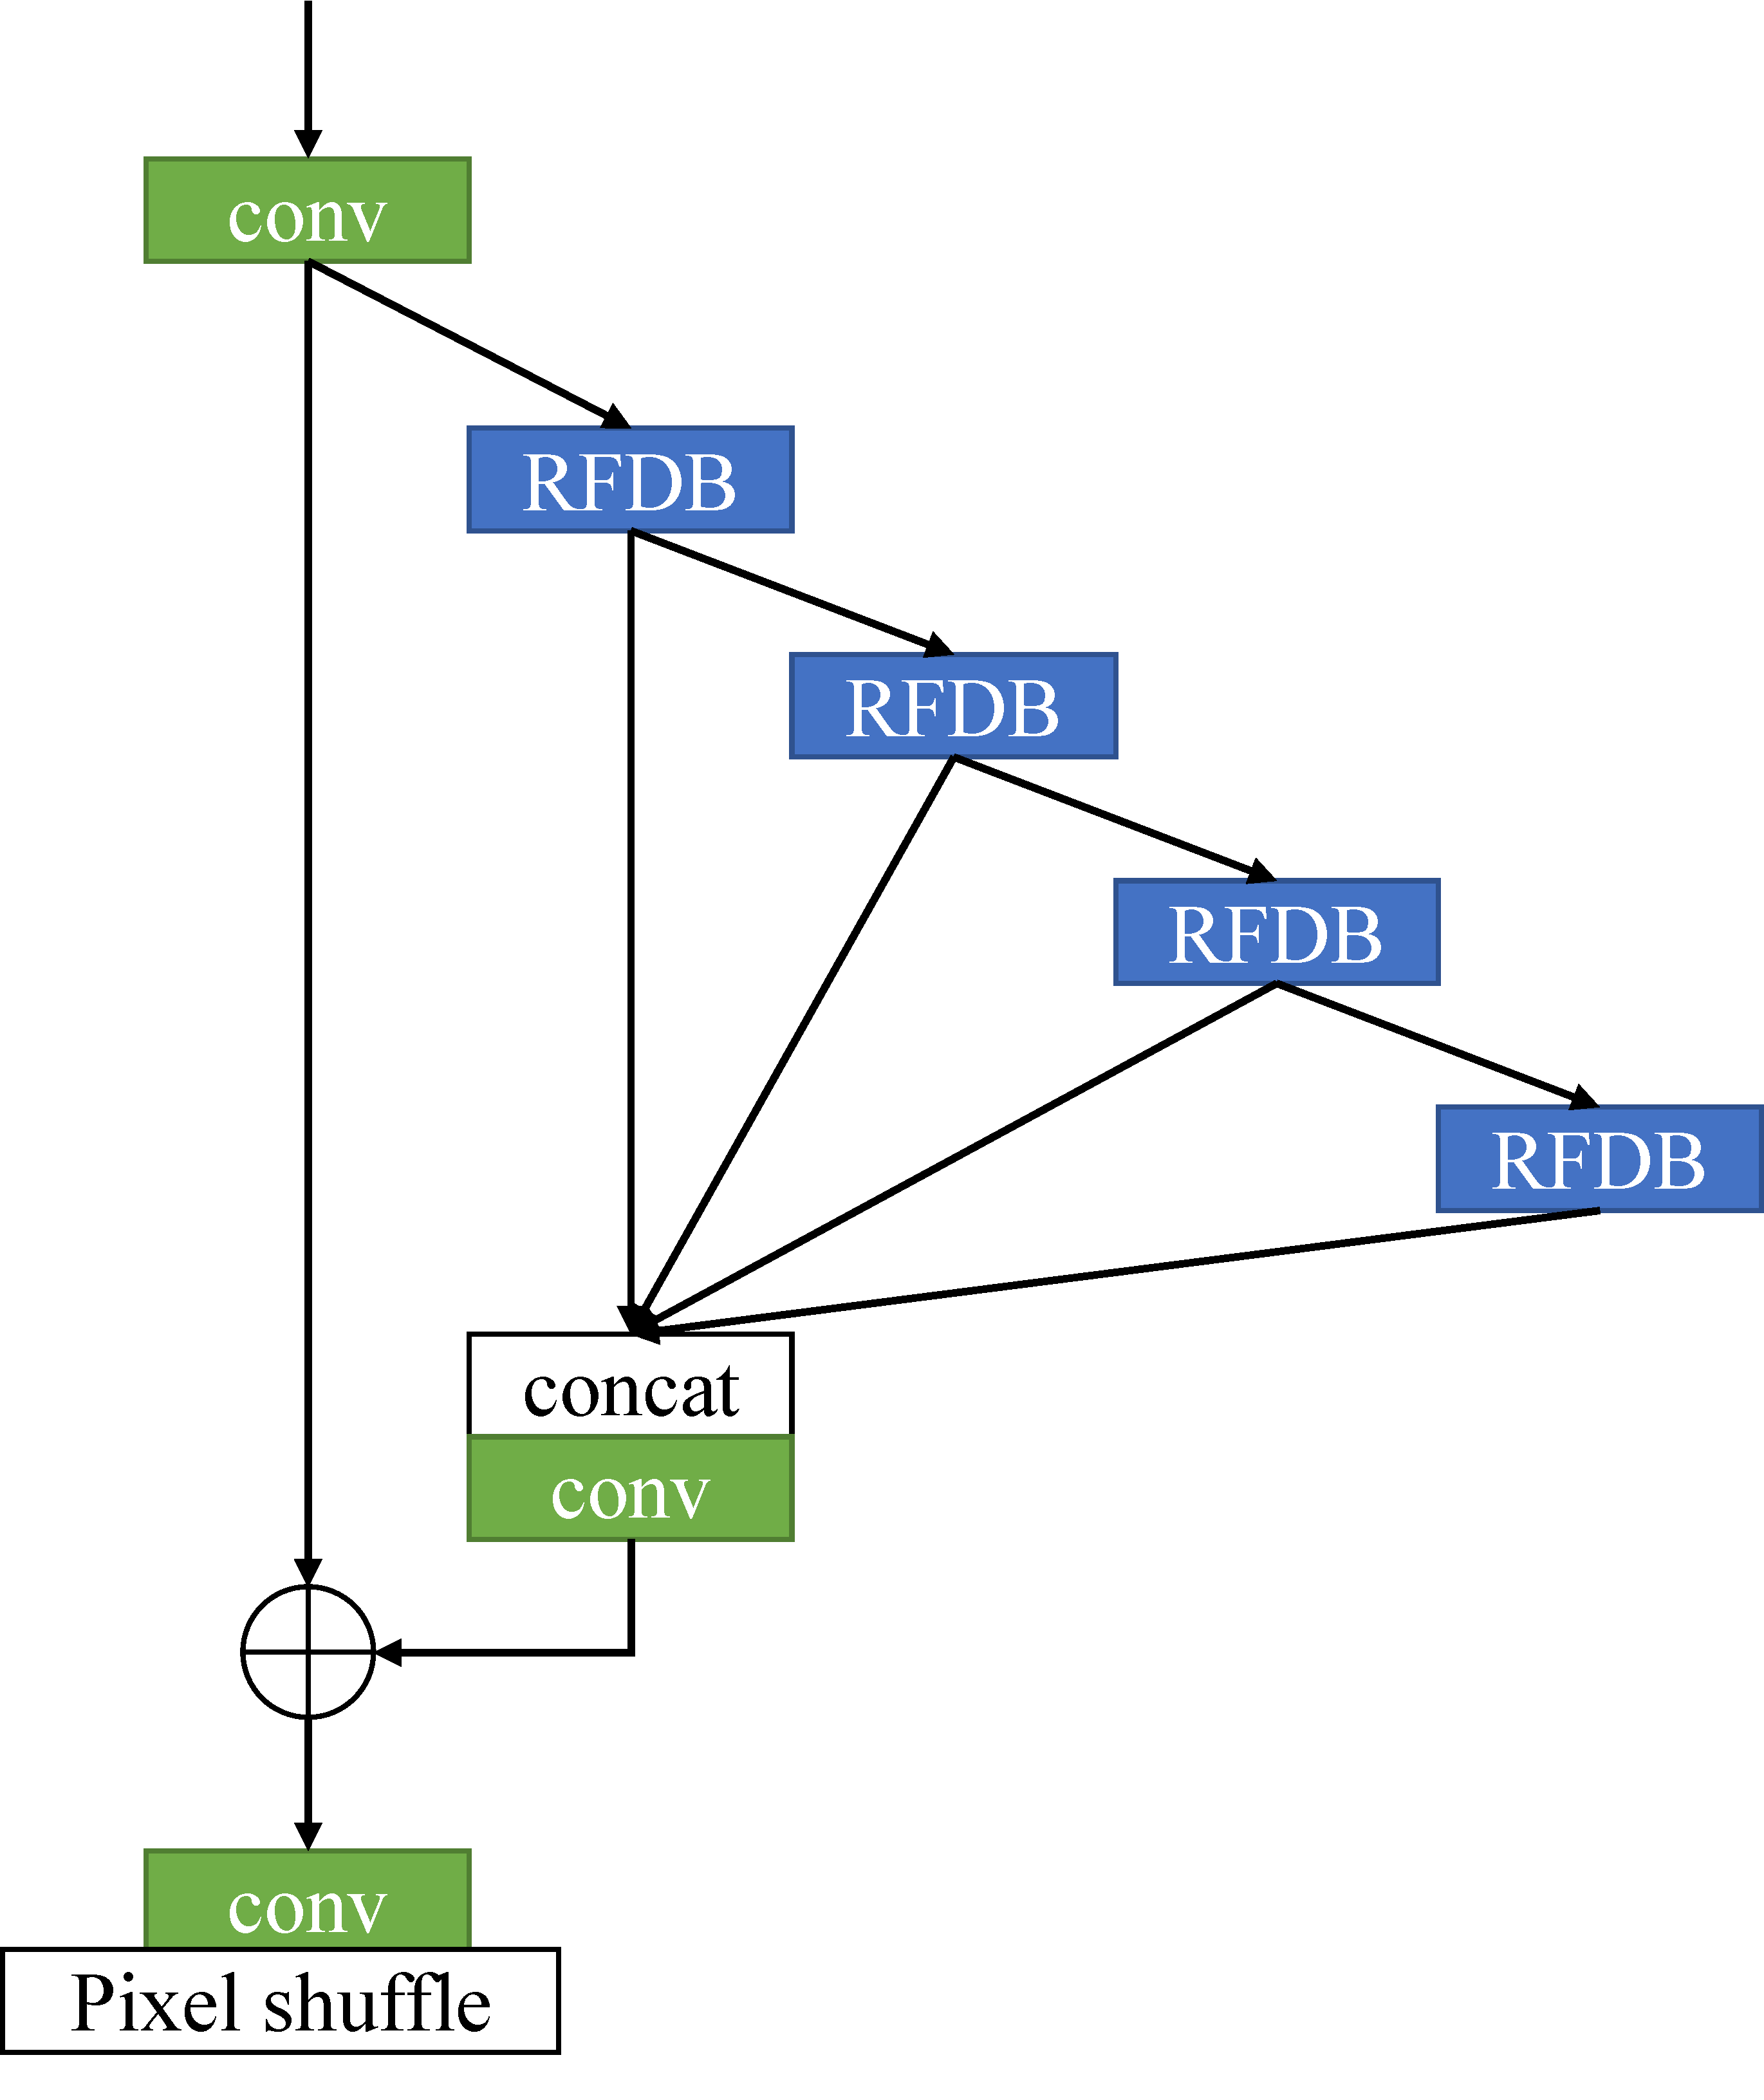
\includegraphics[width=\textwidth]{../RFDN.pdf}
        \caption{RFDN}
        \label{fig:RFDN}
    \end{subfigure}
    \begin{subfigure}[b]{0.49\linewidth}
		\centering
        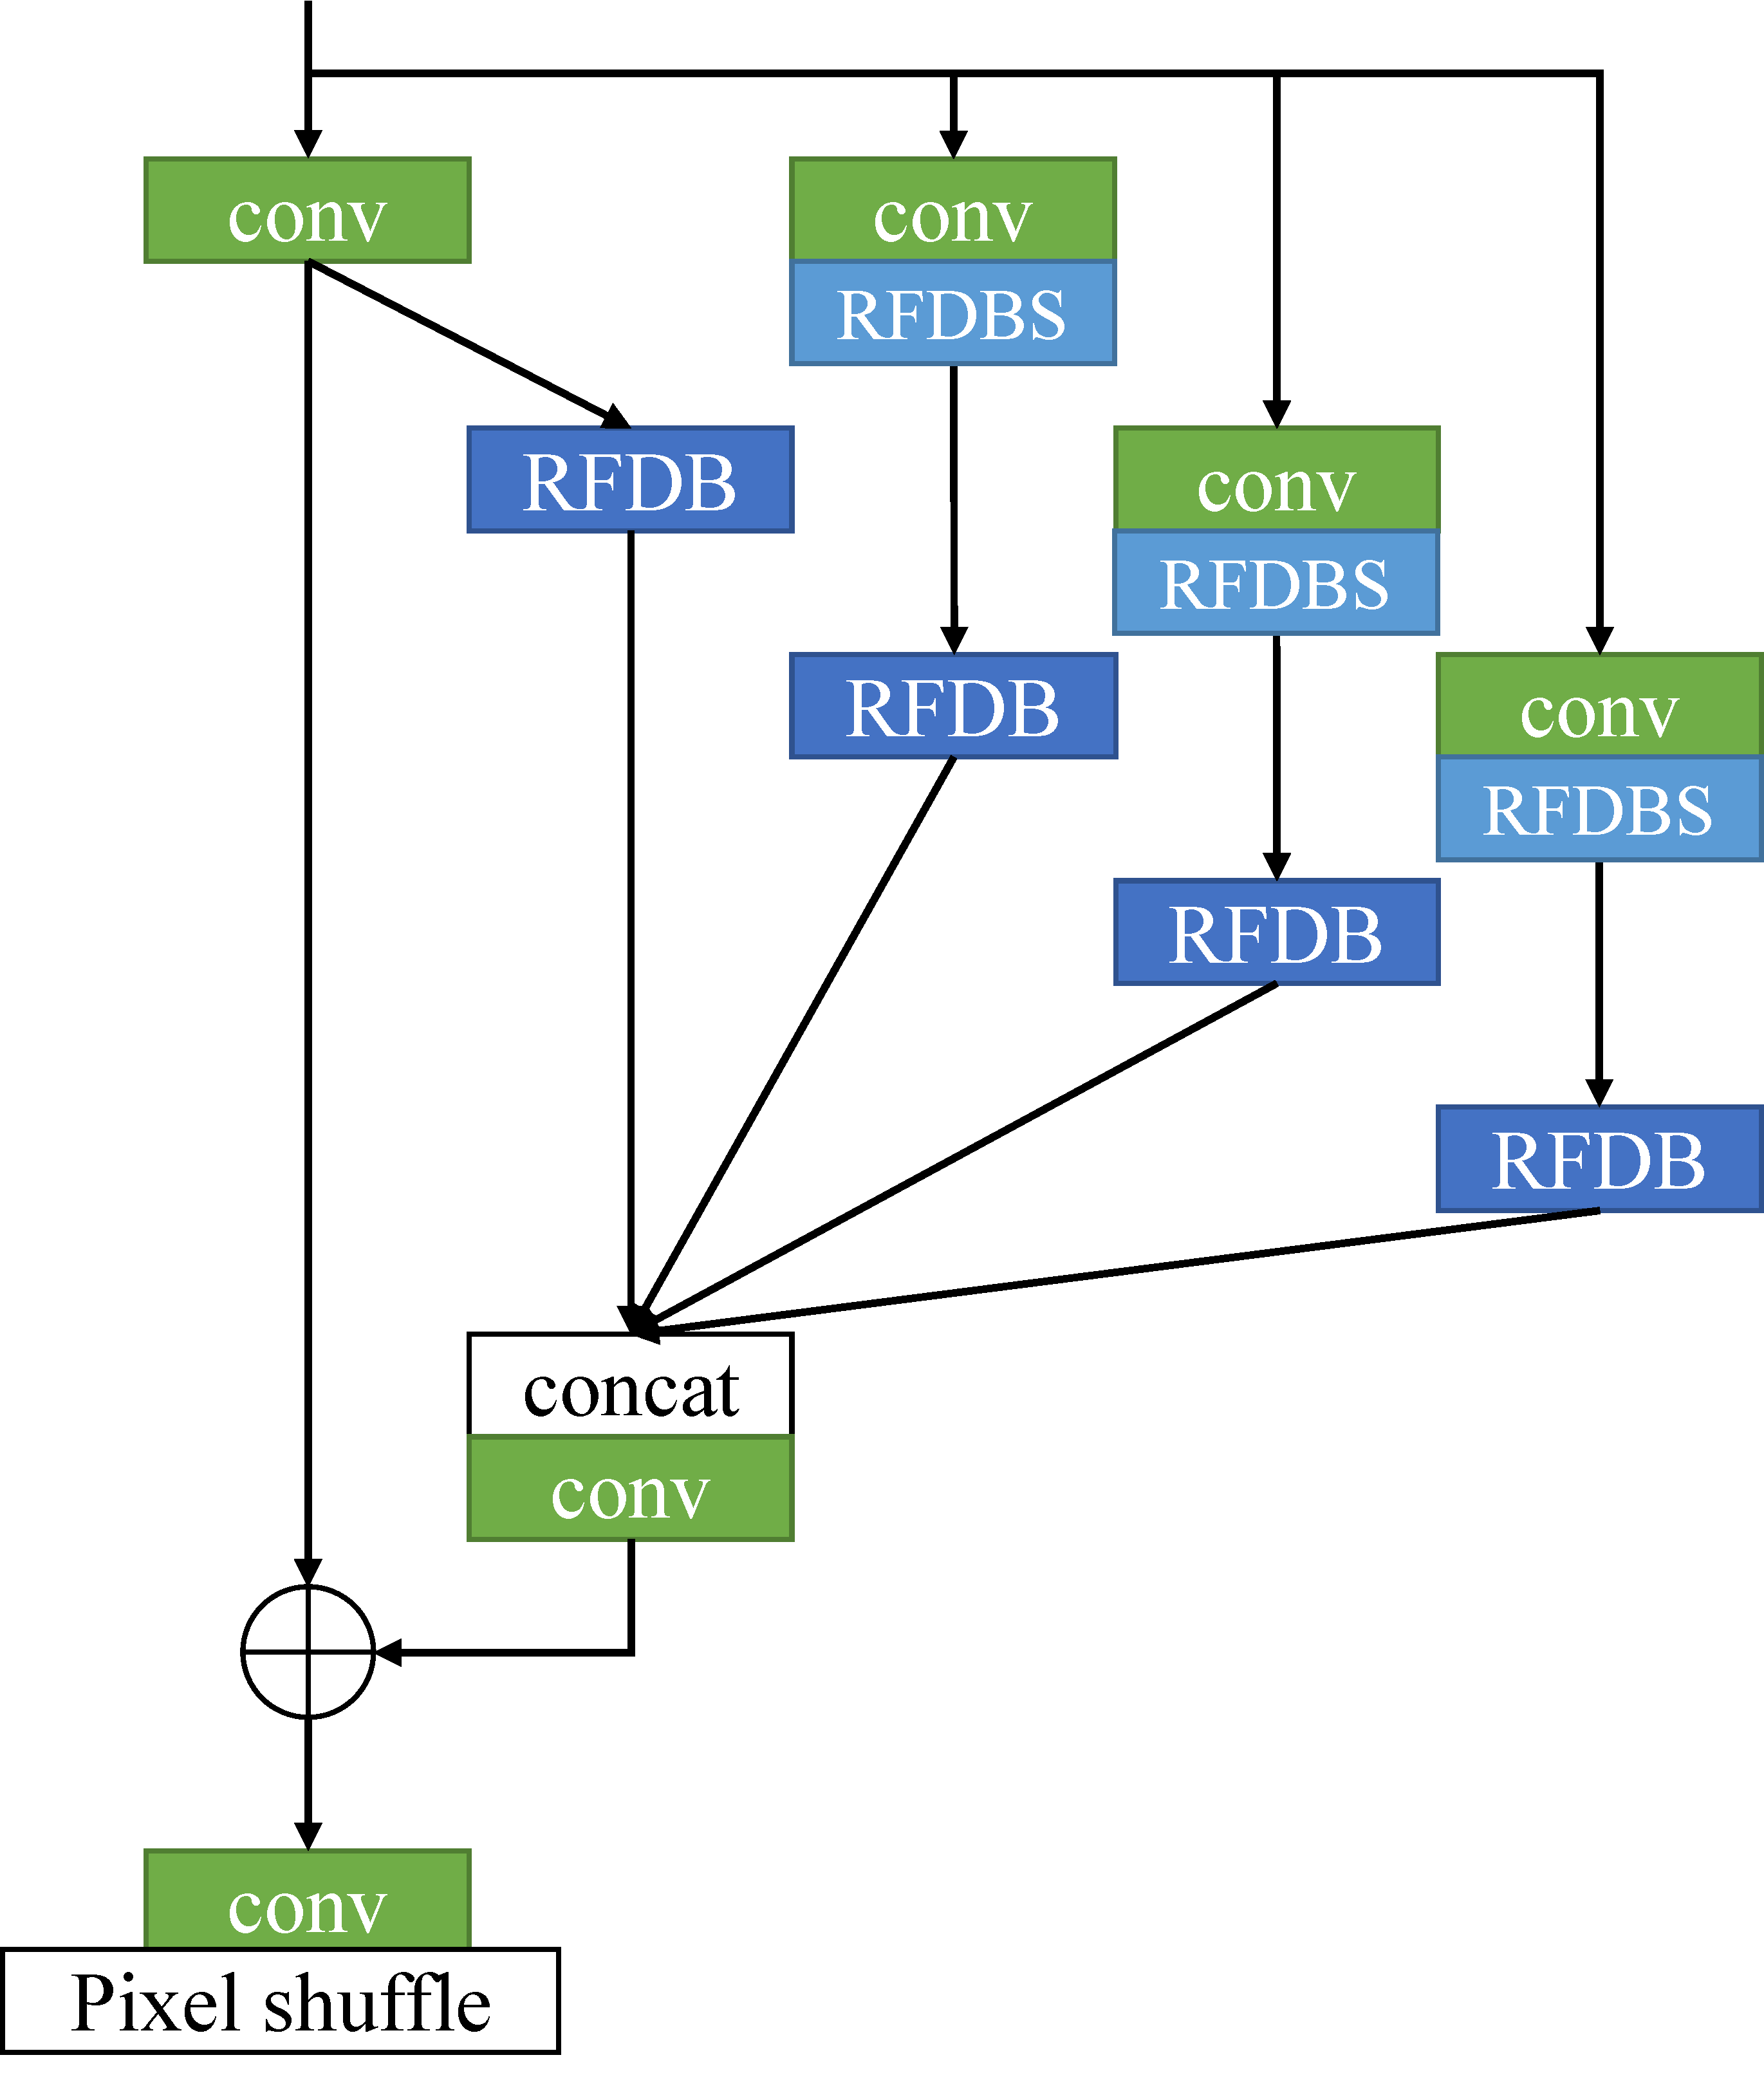
\includegraphics[width=\textwidth]{../Branching.pdf}
        \caption{Branching}
        \label{fig:Branching}
    \end{subfigure}
    \begin{subfigure}[b]{0.49\linewidth}
		\centering
        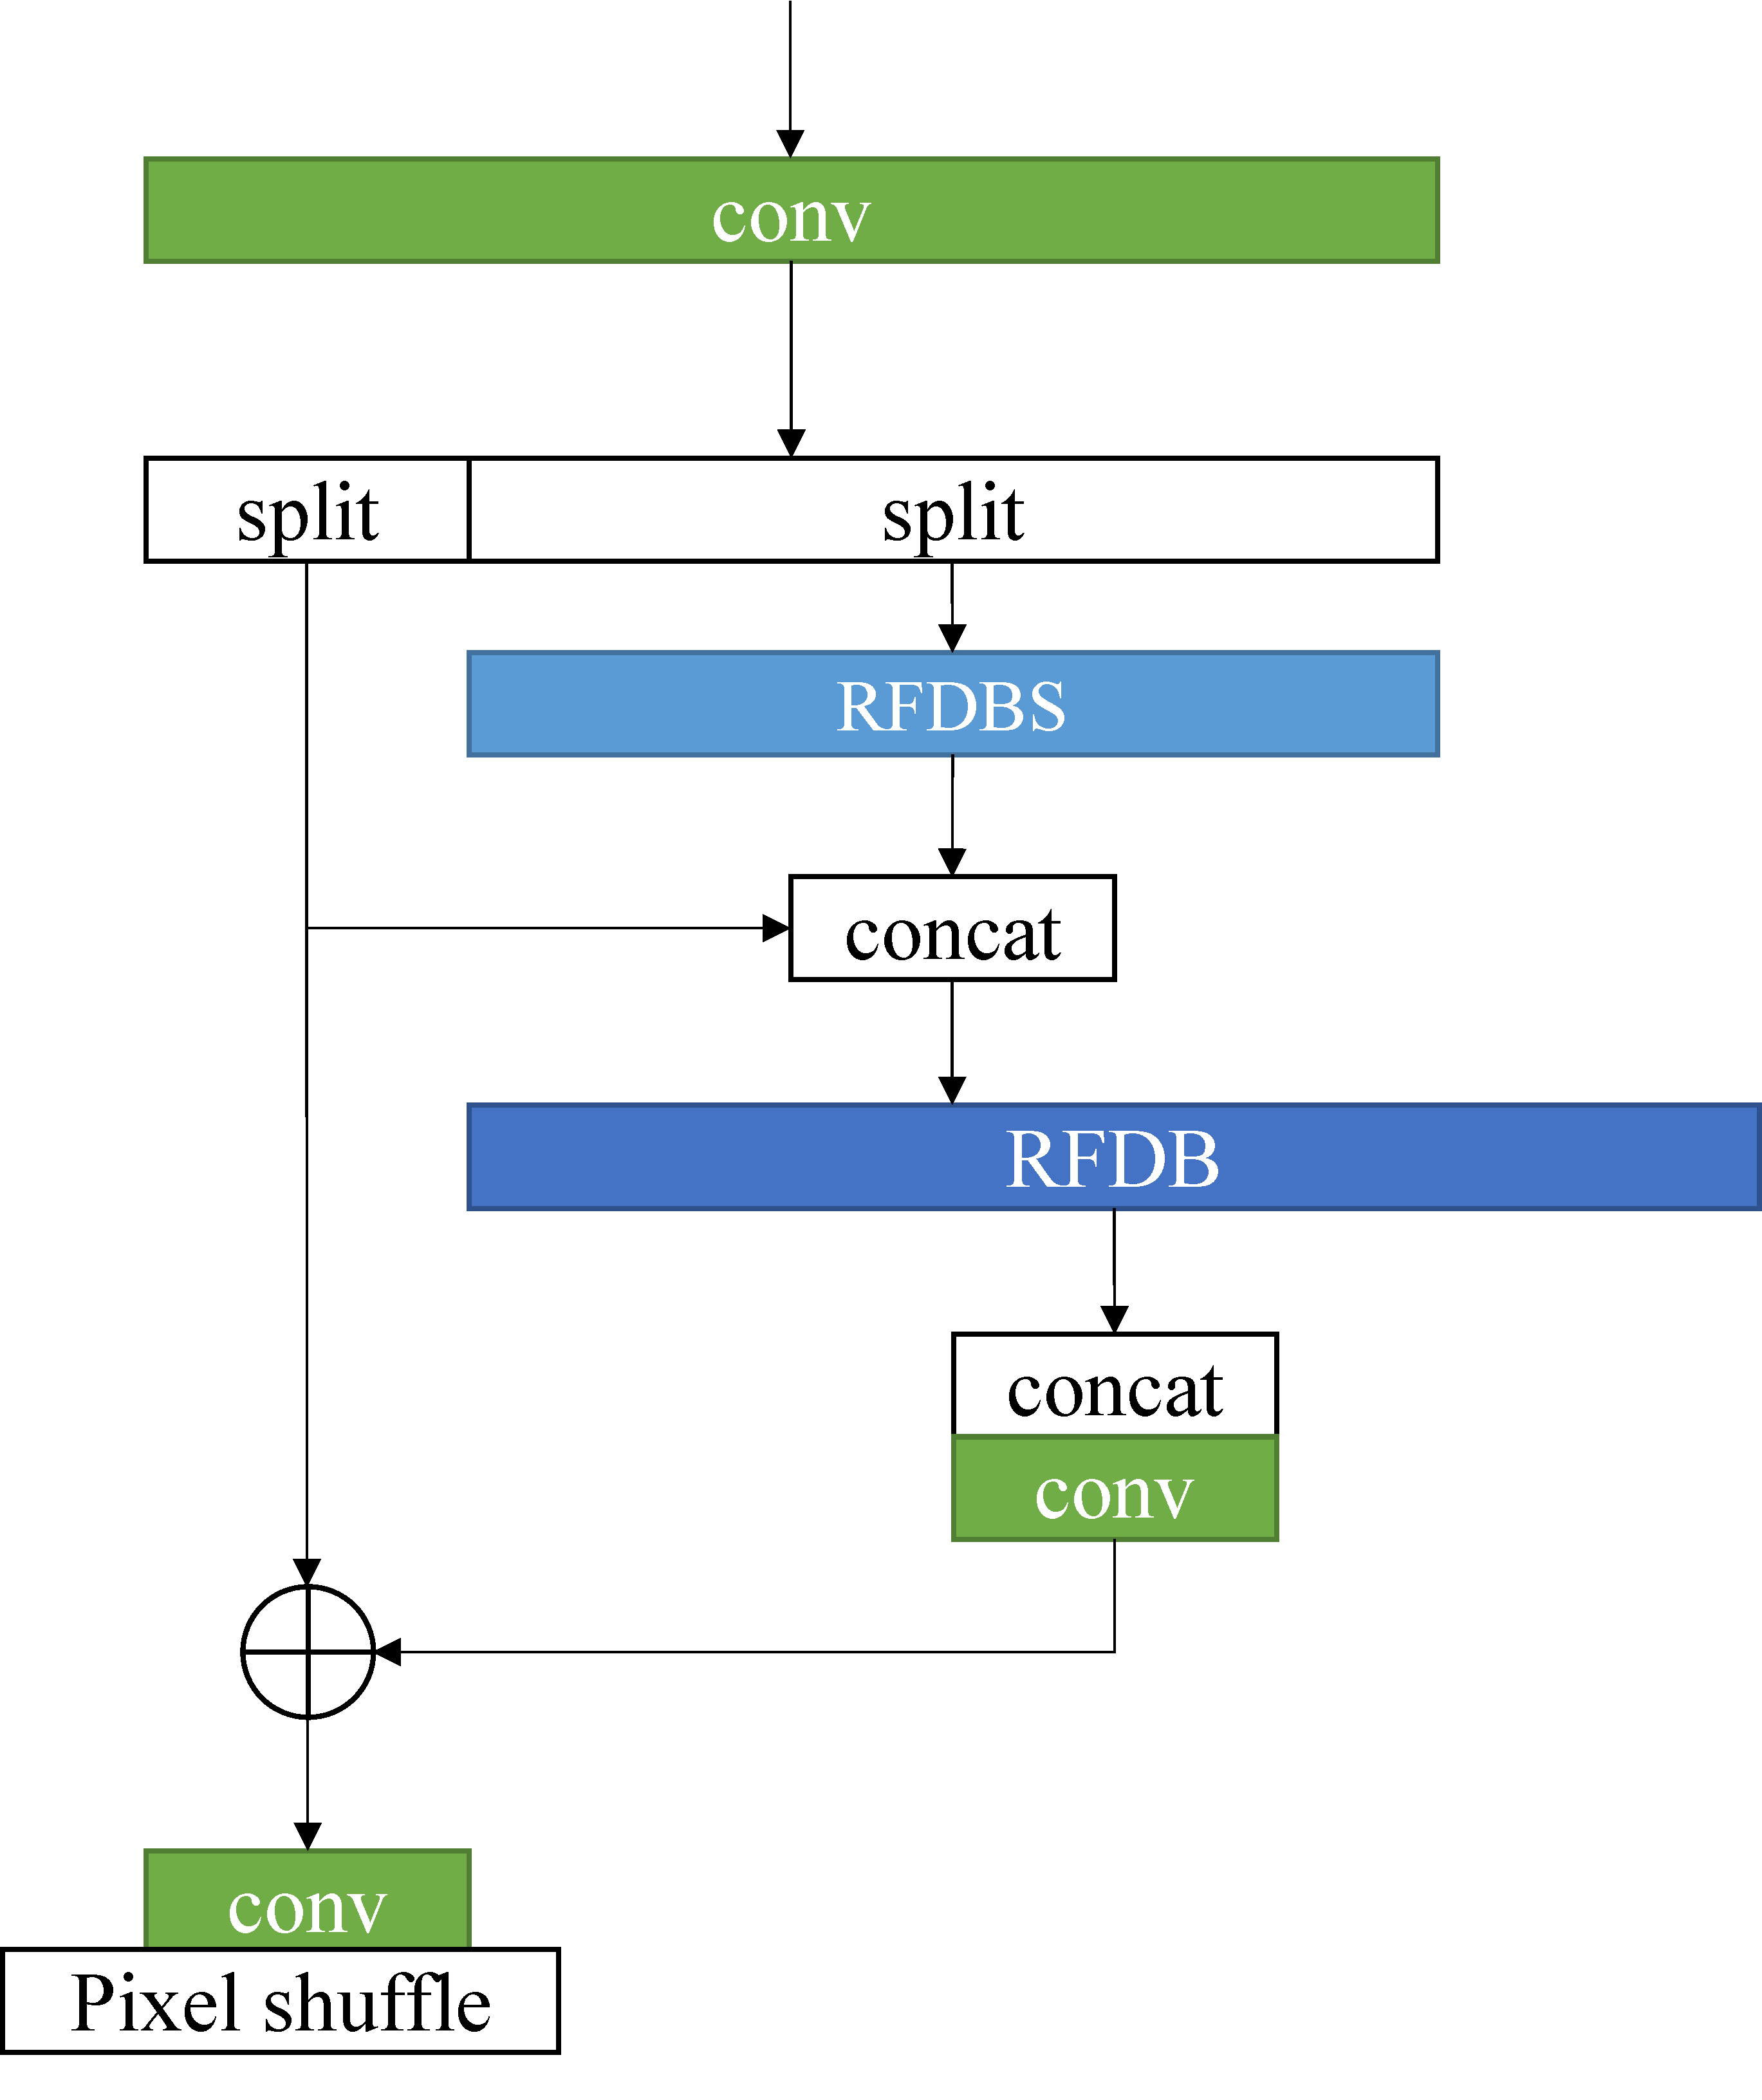
\includegraphics[width=\textwidth]{../Re-parametrization.pdf}
        \caption{Re-parametrization}
        \label{fig:Re-parametrization}
    \end{subfigure}
    \begin{subfigure}[b]{0.49\linewidth}
		\centering
        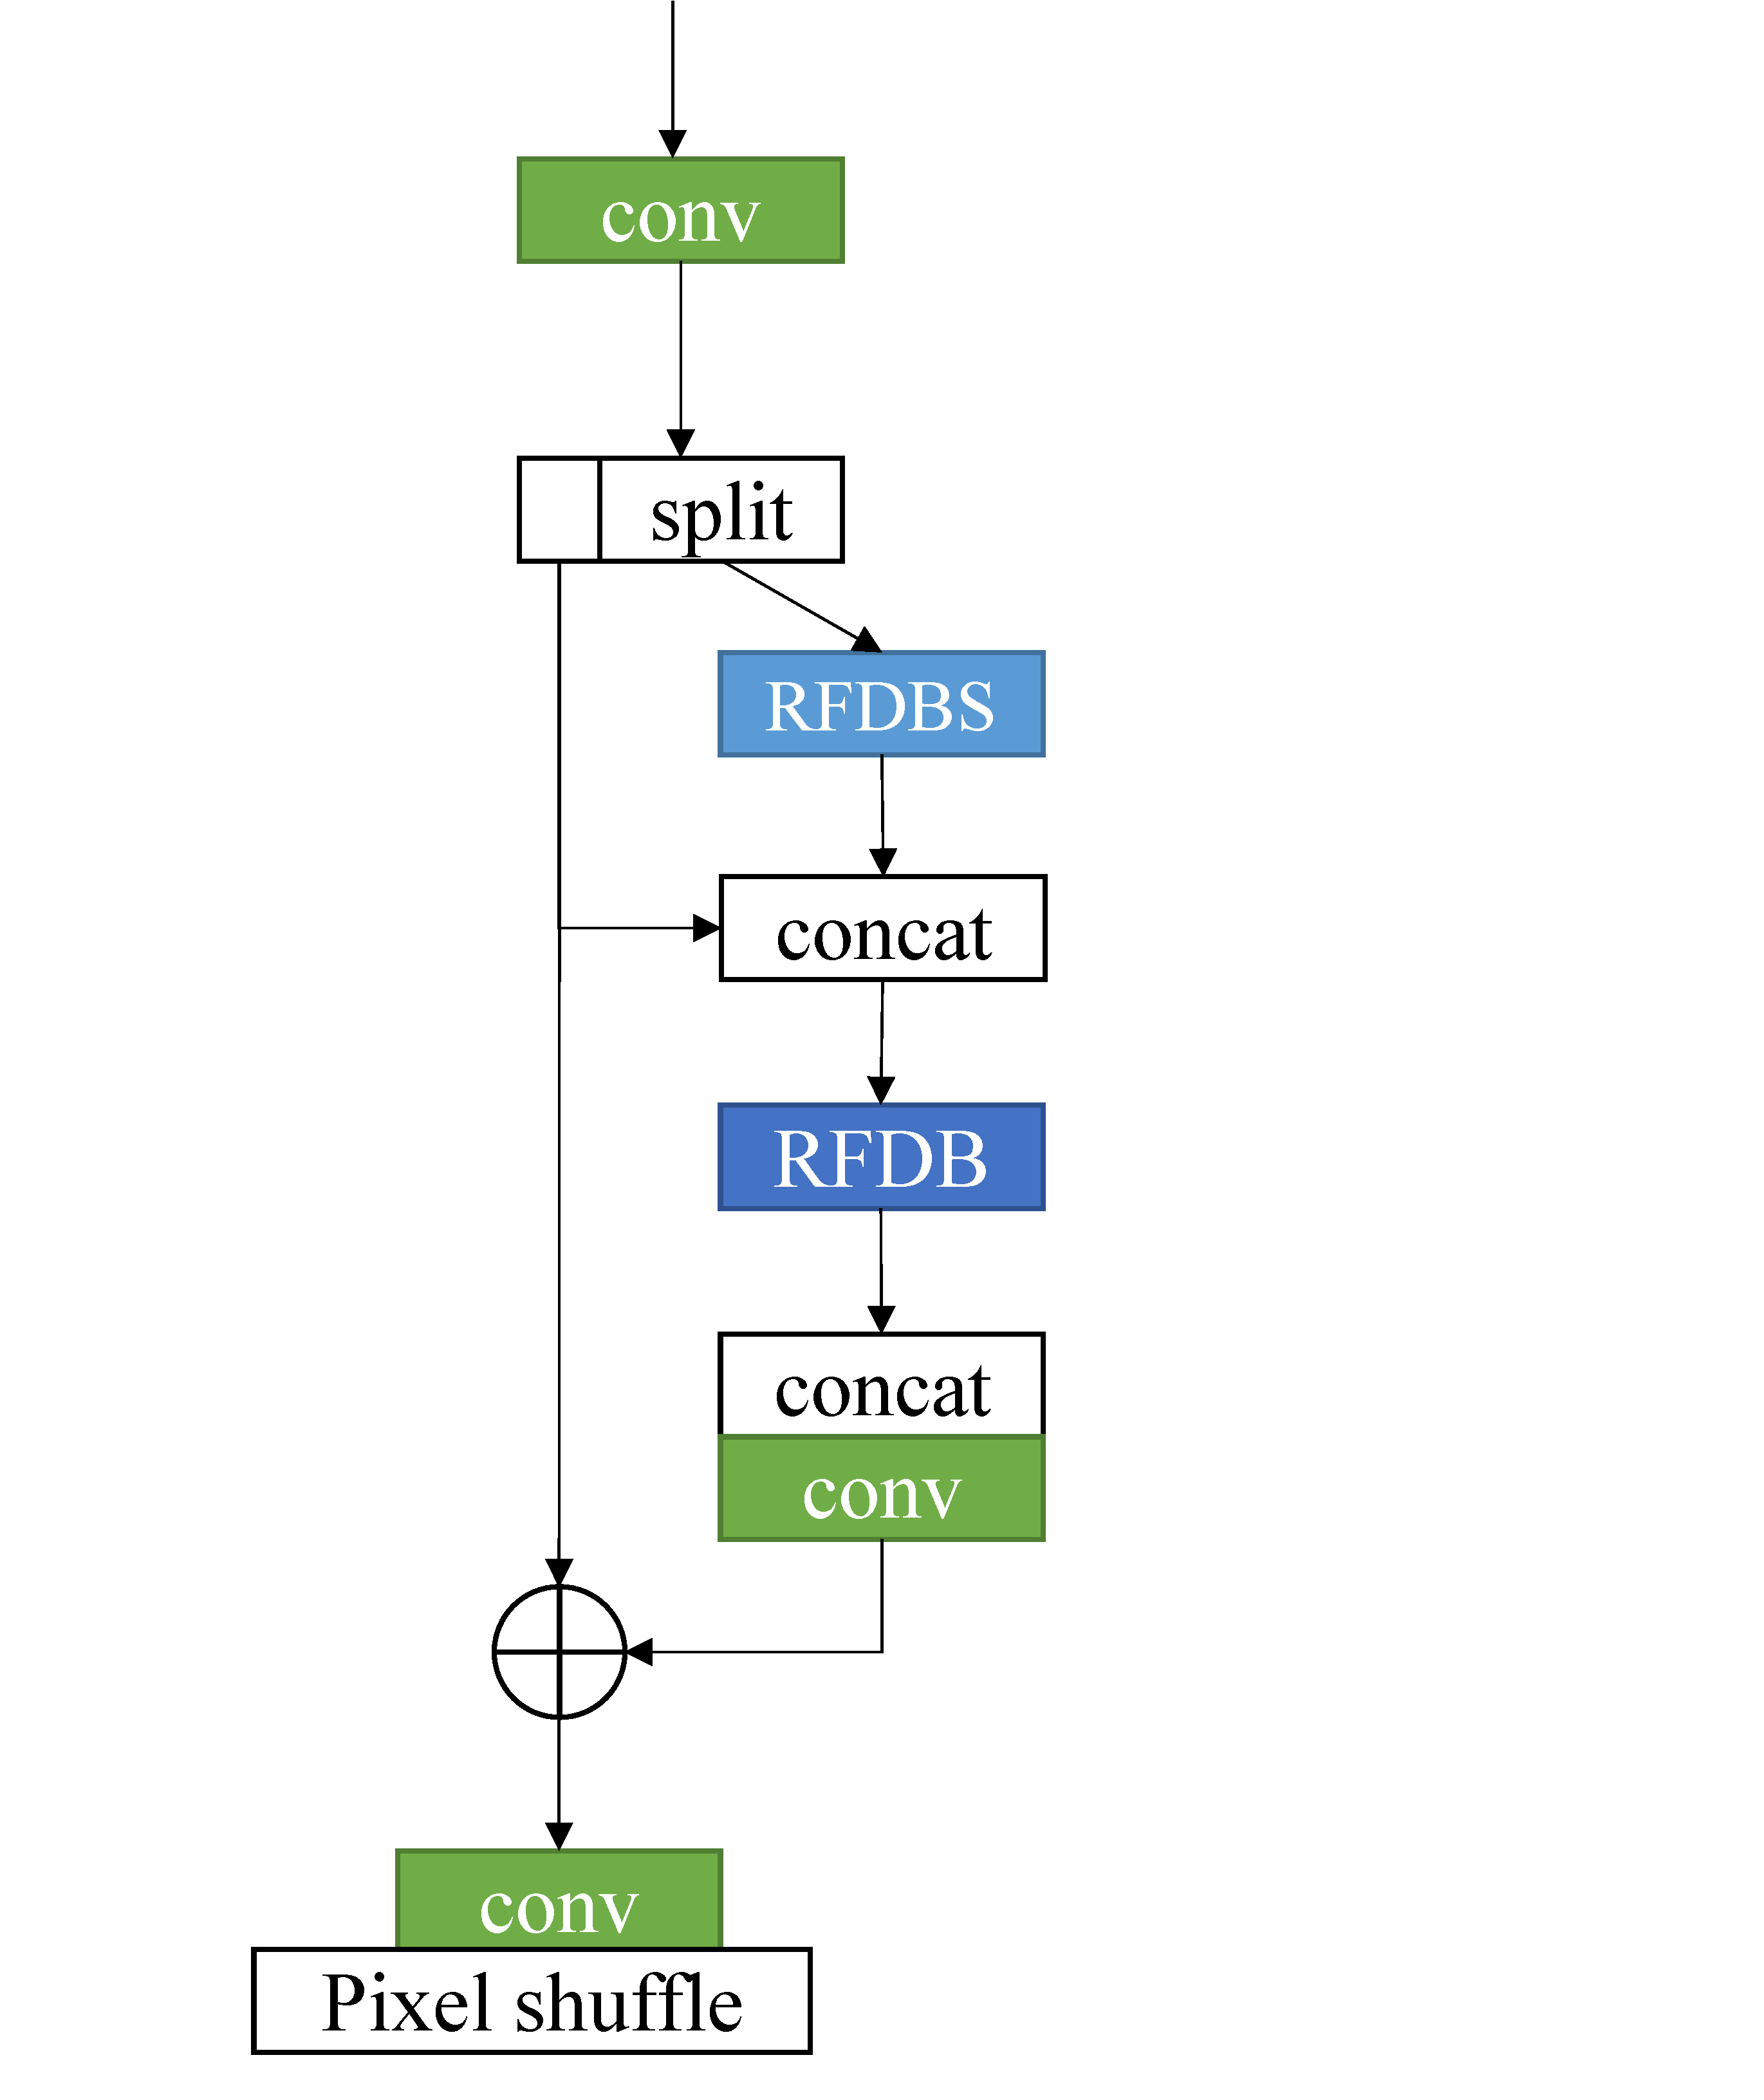
\includegraphics[width=\textwidth]{../Pruning.pdf}
        \caption{Pruning}
        \label{fig:Pruning}
    \end{subfigure}
    \caption{Transform a pre-trained RFDN into PRFDN}
    \label{fig:PRFDN}
\end{figure}

\vspace{4mm}
Please fill the following table specifying the technical information (besides writing it), should take 1 minute. 
%FILL THIS TABLE PLEASE
% Input:         size of the input patch used for TRAINING
% Training time: in hours, how many hours do you train?
% Attention:     Do you use attention mechanisms? If YES, indicate how in the technical details below
% Optimization:  Do you use quantization or prunning?
% Params:        Number of parameters of the model
% GPU:           GPU used in yout experiments

\begin{table}[]
    \centering
    \resizebox{\textwidth}{!}{
    \begin{tabular}{c|c|c|c|c|c|c}
        Input & Training Time & Attention & Quantization & \# Params. (M) & GPU  \\
        \hline
         (256,256,3) & 12h & No & Yes & 5 Million & RTX 3070 8G
    \end{tabular}
    }
    \caption{FILL THIS TABLE PLEASE}
    \label{tab:my_label}
\end{table}

\section{Technical details}
\begin{itemize}
    \item Language: Python
    \item Framework: Pytorch, Torch-Pruning\cite{fang2023depgraph}
    \item Optimizer: AdaM
    \item Learning rate: 1e-5 before re-parametrization, 1e-6 after re-parametrization
    \item GPU: RTX 3070 8G
    \item Datasets for training: LSDIR and DIV2K
\end{itemize}

\vspace{4mm}
\noindent Any particularities of the solution for this competition in comparison to other SR challenges (if applicable).
N/A

\section{Other details}
\begin{itemize}

\item Planned submission of a solution(s) description paper at NTIRE 2023 workshop [YES/ NO].
YES

\item General comments and impressions of the NTIRE 2023 Real-Time Super-Resolution Challenge (we appreciate your feedback to improve in future editions).

Positive impression: Scripts for running the models and measuring metrics are well organized.

Negative impression: Instructions are not clear (e.g. there are some posts in the forum saying that they cannot find the test set, but none of the organizers respond).

A small suggestion: Create a group in instant messaging apps (e.g. Discord or Telegram) for convenient communication.

\item What do you expect from a new challenge in image restoration, enhancement and manipulation?
Real-time video super-resolution; Efficient compressed video restoration.

\end{itemize}


%%%%%%%%% REFERENCES
{\small
\bibliographystyle{ieee_fullname}
\bibliography{egbib}
}
\end{document}